\chapter{Introdução}

\label{CapIntro}

% Resumo opcional. Comentar se não usar.
%\resumodocapitulo{Resumo opcional}

\section{Contextualização}

A Constituição Federal Brasileira, em seu artigo 5º, define:

\begin{quoting}[rightmargin=0cm,leftmargin=4cm]
%\begin{singlespace}
{\footnotesize 
``Art. 5º. Todos são iguais perante a lei, sem distinção de qualquer natureza, garantindo-se aos brasileiros e aos estrangeiros residentes no 
País a inviolabilidade do direito à vida, à liberdade, à igualdade, à segurança e à propriedade[...]''
\\ (Constituição Federal, 1988)\cite{constituicao}.
}
%\end{singlespace}
\end{quoting}

Baseando-se na igualdade proposta e elevando este conceito acima do nível simplesmente nacional, são propostas frequentemente novas tecnologias que buscam proporcionar 
ou ampliar habilidades funcionais de pessoas com deficiência, garantindo autonomia e igualdade em questão de acessibilidade a estas pessoas, promovendo por 
fim a sua independência e inclusão. Para se referir a este tipo de tecnologias, é comumente utilizado o termo Tecnologia Assistiva - TA \cite{bersch2008introduccao}.  

Sancionado em 2015, o Estatudo da Pessoa com Deficiência fornece uma definição para acessibilidade no âmbito nacional:

\begin{quoting}[rightmargin=0cm,leftmargin=4cm]
%\begin{singlespace}
{\footnotesize 
``I - acessibilidade: possibilidade e condição de alcance para utilização, com segurança e autonomia, de espaços, mobiliários, equipamentos urbanos, 
edificações, transportes, informação e comunicação, inclusive seus sistemas e tecnologias, bem como de outros serviços e instalações abertos ao público,
de uso público ou privados de uso coletivo, tanto na zona urbana como na rural, por pessoa com deficiência ou com mobilidade reduzida;''\\
(Estatuto Da Pessoa com Deficiência, 2015)\cite{estatutodef}.
}
%\end{singlespace}
\end{quoting}

Assim, pessoas com deficiência motora, que têm em sua condição uma autonomia reduzida, possuem também uma menor acessibilidade geral, sendo necessário fornecer
meios de ampliar sua independência, respeitando os seus direitos fundamentais. A autonomia em questão é afetada diretamente pelo tipo de lesão ou 
má-formação observada: a paraplegia, ou ausência de membros inferiores, dificulta  locomoção, já a tetraplegia chega a restringir quase toda a movimentação do deficiente.
Na pesquisa por novas Tecnologias Assistivas para incrementar a autonomia nestes casos, há o ramo de desenvolvimento de braços mecânicos assistivos, podendo 
estes serem fixos em determinado local, ou móveis, como quando são acoplados em cadeiras de rodas. Enquadrando-se na categoria de TA de auxílio para vida
diária e vida prática, os braços robóticos montados sobre cadeiras de rodas (\textit{WMRA - Wheelchair Mounted Robotic Arm}), assim como outras tecnologias 
assistivas, têm como finalidade permitir um bom desempenho em atividades diárias básicas (\textit{ADL} - Activities of Daily Living) \cite{capille2010kinematic}. 

Tendo em vista que, em 2010, 15\% da população mundial vivia com algum tipo de deficiência \cite{world2011world}, os avanços buscados em tecnologias 
assistivas são de grande importância, pois afetam grande parte da população, direta e indiretamente, 
garantindo maior liberdade a pessoas com deficiência e uma sociedade
mais igualitária, alinhando-se com a agenda 2030 da ONU - Organização das Nações Unidas,
para desenvolvimento sustentável, especificamente com a meta 10 - Redução das Desigualdades \cite{un2030agenda}.

\section{Definição do problema}

Foi idealizada e construída na Universidade de Brasília - UnB, no período de 2018 a 2019, 
a estrutura mecânica de um braço robótico a ser montado em uma cadeira de rodas, com a finalidade de ser
uma solução barata e suficiente para aprimorar a acessibilidade de pessoas que sofreram lesão medular completa do tipo tetraplegia \cite{fernando2019assistivo}. 
O projeto base conta com uma seleção inicial de atuadores para as juntas deste, no entanto, para garantir uma adequação real do braço construído como 
tecnologia assistiva, faz-se necessário que o braço possa ser controlado pelo usuário final, sendo essencial para isto a verificação dos atuadores selecionados, 
inserção de elementos sensoriais no manipulador, projeto de uma plataforma de comando e junção eletro-eletrônica desta com os atuadores e sensores propostos.

\subsection{Estrutura do manipulador robótico base}
\label{sec:EstruturaBase}

O braço robótico em questão é do tipo articulado, possui 3 juntas principais e um pulso implementado como 3 juntas rotativas com eixos que não se cruzam em um
mesmo ponto. A primeira junta constitui a rotação do robô em torno de sua base, sendo considerada como a junta do quadril, a segunda é denominada como ombro, a terceira como cotovelo e as juntas do 
pulso são divididas com base no tipo de movimento de rotação que causam, sendo estes denominados como \textit{yaw}, \textit{pitch} e \textit{roll}. As juntas do robô são 
construídas majoritariamente de chapas de alumínio cortadas e dobradas, os elos por sua vez foram projetados com material PVC e \textit{Nylon (TechNyl)}. 

Foram selecionados para o acionamento do manipulador 3 motores do tipo Mabuchi JC/LC-578VA, 1 motor de passo HT23-397/NEMA 23 e 2 motores de passo 
42HS48-1684/NEMA 17. Para a transmissão do torque de saída dos atuadores propostos até o ponto de atuação foi idealizada uma transmissão por engrenagens,
sendo as engrenagens fabricadas com tecnologia de manufatura aditiva e materiais PLA e ABS. Para o comando do robô foi proposto inicialmente um Arduino, 
no entanto, esta escolha deve ser revista após a revisão dos atuadores e seleção de sensores e circuitos de ativação e processamento. 

A modelagem gráfica do manipulador pode ser vista na figura \ref{fig:manipulador-base}.

\begin{figure}[h]
\caption{Modelagem do robô montado \cite{fernando2019assistivo}.}    
\begin{centering}
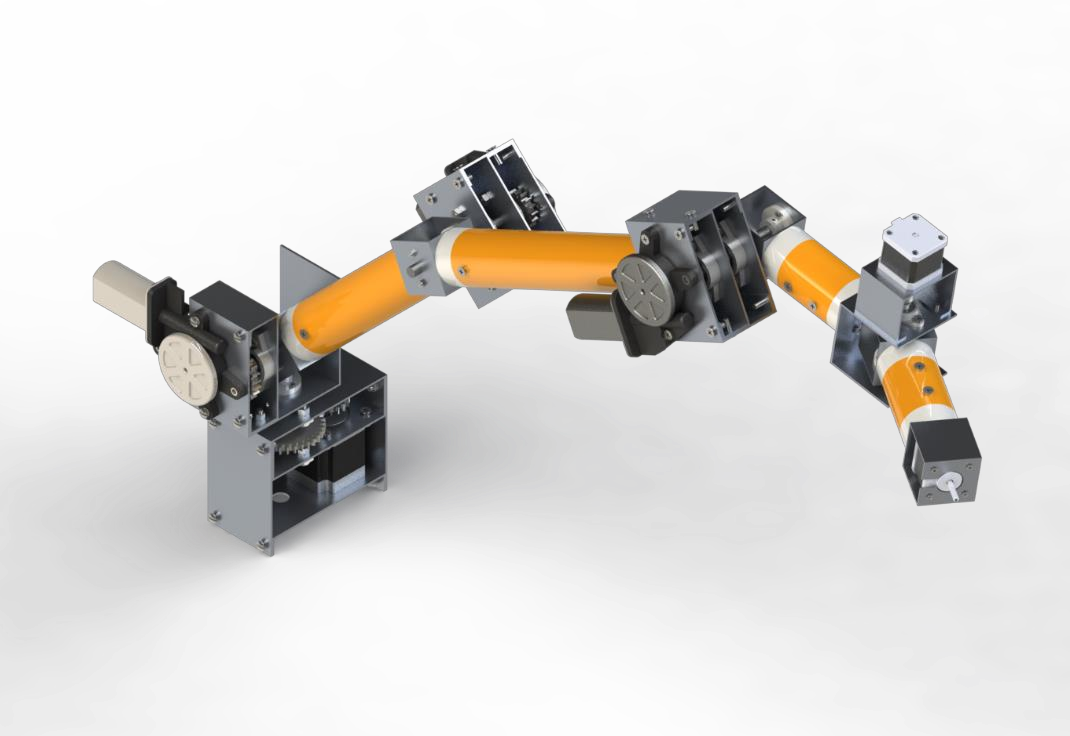
\includegraphics[width=0.8\columnwidth]{images/intro/manipulador-base.png}
\par\end{centering}

\label{fig:manipulador-base}
\end{figure}

Nota-se pela figura o local de aplicação dos atuadores selecionados, assim como descrito na tabela \ref{tab:AtuadoresPre}. A figura demonstra também como
foram empregados os tubos de material PVC e acopladores de \textit{Nylon} na construção dos elos, bem como o formato das juntas com uma separação para inserção
das engrenagens que compõem as reduções calculadas no projeto base \cite{fernando2019assistivo}. Maiores dados sobre os motores serão
fornecidos ao longo do desenvolvimento do texto, como na tabela \ref{tab:Motores}, que indica suas condições elétricas de funcionamento
e tabela \ref{tab:Analise-Torque}, que indica os torques fornecidos pelos motores. Todos os dados sobre os atuadores foram retirados
de seus \textit{datasheets}, incluídos no anexo \ref{anexo-datasheets} deste documento.

\begin{table}[h]
\begin{centering}  

\begin{tabular}{|c|c|}
    \hline
    Junta & Atuador selecionado \tabularnewline
    \hline
    \hline
    1 (Base) & Motor de passo HT23-397/NEMA 23 \tabularnewline
    \hline
    2 (Ombro) & Motor DC Mabuchi JC/LC-578VA \tabularnewline
    \hline
    3 (Cotovelo) & Motor DC Mabuchi JC/LC-578VA \tabularnewline
    \hline
    4 (\textit{Pitch}) & Motor DC Mabuchi JC/LC-578VA \tabularnewline
    \hline
    5 (\textit{Yaw}) & Motor de passo 42HS48-1684/NEMA 17 \tabularnewline
    \hline
    6 (\textit{Roll}) & Motor de passo 42HS48-1684/NEMA 17 \tabularnewline
    \hline
\end{tabular}

\caption{Atuadores pré-selecionados para as juntas \cite{fernando2019assistivo}.}
\label{tab:AtuadoresPre}

\par\end{centering}
\end{table}

\section{Objetivos do projeto}

O objetivo principal deste trabalho é analisar o braço robótico apresentado na seção \ref{sec:EstruturaBase} a fim de revisar os atuadores existentes neste e
propor instrumentos de medição e circuitos de acionamento e processamento para serem inseridos em sua estrutura, bem como idealizar um controlador para reger 
os movimentos deste manipulador robótico. 
Os circuitos eletro-eletrônicos e o sistema de acionamento propostos devem
ser capazes de receber comandos do usuário e acionar os atuadores de 
maneira a permitir que a estrutura mecânica subjacente e o efetuador 
final do manipulador sejam posicionados de modo a auxiliar o operador 
na interação com o espaço ao seu redor para a realização de atividades
diárias básicas.

Pautando-se em um dos objetivos do trabalho base, o manipulador, com 
todo o sistema de sensoriamento, ativação e comando, deve apresentar 
um baixo custo, para que possa ser considerado um protótipo acessível
para auxílio de pessoas com deficiência motora dos membros inferiores 
e superiores.

% Escrever sobre metodologia? 
%\section{Metodologia de desenvolvimento}

\section{Apresentação do trabalho}

O trabalho foi organizado em 6 capítulos. O primeiro capítulo é 
introdutório, indicando as motivações e objetivos do projeto. 
No Capítulo 2 é apresentada uma revisão bibliográfica sobre projetos
semelhantes, da mesma forma são expostos modelos comerciais de WMRAs, 
servindo como possíveis fontes de inspiração e comparação com o produto 
a ser desenvolvido neste trabalho. No mesmo capítulo são também revisados
conceitos teóricos que forneceram o embasamento técnico para a 
realização do projeto. 

O desenvolvimento foi dividido em 2 capítulos, Capítulo 3, onde
são enunciados os objetivos, diretrizes e escolhas realizadas quanto 
ao desenvolvimento dos diversos circuitos eletro-eletrônicos, e 
Capítulo 4, que descreve a maneira como o controlador geral do robô foi
implementado.

O Capítulo 5 contém resultados observados ao longo do desenvolvimento,
tanto obtidos por simulações como através de protótipos construídos, 
para comparação entre os objetivos propostos e resultados de fato obtidos.
No Capítulo 6 encontram-se as considerações finais do projeto, com 
uma conclusão pautada em tudo o que foi observado durante a realização
do projeto e perspectivas futuras para possíveis trabalhos que possam 
emanar do projeto desenvolvido. 